\documentclass[UTF8,zihao=-4]{ctexart}

\usepackage[a4paper,margin=2.5cm]{geometry}
\usepackage{amsmath,amssymb,bm}
\usepackage{siunitx}
\usepackage{graphicx}
\usepackage{booktabs}
\usepackage{threeparttable}
\usepackage{subcaption}
\usepackage{float}
\usepackage[section]{placeins}
\usepackage{xcolor}
\usepackage{setspace}
\usepackage{microtype}
\usepackage[
  backend=biber,
  style=numeric,
  sorting=none,
  giveninits=true
]{biblatex}
\usepackage[
  colorlinks=true,
  linkcolor=blue!55!black,
  citecolor=green!40!black,
  urlcolor=blue!60!black
]{hyperref}
\usepackage[nameinlink,noabbrev]{cleveref}

\addbibresource{bibliography.bib}
\graphicspath{{../figures/}}

\setstretch{1.25}
\setlength{\parindent}{2em}
\setlength{\parskip}{0.25em}
\setlength{\textfloatsep}{12pt plus 2pt minus 2pt}
\setlength{\floatsep}{10pt plus 2pt minus 2pt}
\setlength{\intextsep}{10pt plus 2pt minus 2pt}

\crefname{figure}{图}{图}
\crefname{table}{表}{表}
\crefname{section}{节}{节}
\crefname{equation}{式}{式}

\newcommand{\alphaRatio}{\alpha=J_2/J_1}
\newcommand{\betaRatio}{\beta=J_3/J_1}
\newcommand{\Ostr}{O_{\mathrm{str}}}
\newcommand{\todo}[1]{\textcolor{red!70!black}{[待补：#1]}}

\title{自旋 $\frac{1}{2}$ 五聚体 Heisenberg 链的临界关联、弦关联与低能激发}
\author{作者姓名}
\date{\today}

\begin{document}

\maketitle

\begin{abstract}
本文研究具有五站点单胞的一维自旋 $\frac{1}{2}$ Heisenberg 链。
在固定 $\beta=0.5$ 的参数截面上，我们结合孤立五聚体精确对角化、
密度矩阵重整化群、弦关联、边缘磁化、纠缠谱和动力学结构因子，
分析不同耦合区域的低能性质。当前有限尺寸证据支持由 $\alpha=0$
特殊解耦点分隔的两个临界区域：负 $\alpha$ 区域同时具有代数体关联、
缓慢衰减的弦关联和局域边缘响应，正 $\alpha$ 区域表现为以
$q=\pi$ 为主的常规无隙反铁磁关联。正侧两个响应峰目前更符合有限尺寸
交叉尺度，而不是额外相的独立边界。负侧是否可以严格分类为无隙
对称性保护拓扑区域，仍需更大尺度动力学计算和虚空间投影对称表示。
\end{abstract}

\noindent\textbf{关键词：}
五聚体自旋链；弦关联；临界态；边缘态；密度矩阵重整化群；动力学结构因子

\tableofcontents

\section{引言}

团簇化量子自旋链为研究局域多重态、量子临界性、隐藏弦关联和边缘自由度之间的
关系提供了可控平台。已有四聚体链研究建立了“孤立单胞多重态—弦关联—纠缠结构—
动力学结构因子”的证据组织方式，并展示了不同耦合区域的低能激发特征
\cite{li2026tetramer}。然而，五聚体单胞包含奇数个自旋 $\frac{1}{2}$，
其低能自由度和 Lieb--Schultz--Mattis 类型约束与偶数自旋单胞不同，因此不能
直接移植四聚体链的相名、弦算符端点或准粒子命名。

本文考虑具有两个胞内耦合 $J_1,J_2$ 和胞间耦合 $J_3$ 的五聚体
Heisenberg 链。我们首先分析孤立五聚体的低能多重态，然后在固定
$\beta=J_3/J_1=0.5$ 的截面上计算基态能量、普通自旋关联、弦关联、
边缘磁化、纠缠谱和动力学结构因子。分析的核心问题包括：

\begin{enumerate}
  \item 负 $\alpha$ 区域是否为普通有隙 Haldane-like 区域；
  \item 正 $\alpha$ 区域内部的两个响应峰是否定义额外相；
  \item $\alpha=0$ 两侧的低能多重态、弦关联和动量结构如何变化；
  \item 负侧的边缘和弦特征能否与临界体关联共存。
\end{enumerate}

当前结果表明，$\alpha=0$ 两侧均具有代数体关联，但负侧同时保留明显更慢的
弦关联衰减和局域边缘响应。我们因此将其保守地称为具有弦与边缘特征的临界区域，
而不提前命名为普通有隙 SPT 相或确定的 gapless SPT 相。

\todo{补充更广泛的五聚体链、无隙 SPT 和团簇自旋链文献。}

\section{模型与数值方法}

\subsection{五聚体 Heisenberg 链}

每个单胞包含五个自旋 $\frac{1}{2}$。以 $n$ 表示单胞编号，
$a=1,\ldots,5$ 表示胞内位置，哈密顿量写为
\begin{align}
H={}&J_1\sum_n
\left(
\bm S_{n,2}\cdot\bm S_{n,3}
+\bm S_{n,3}\cdot\bm S_{n,4}
\right)
\nonumber\\
&+J_2\sum_n
\left(
\bm S_{n,1}\cdot\bm S_{n,2}
+\bm S_{n,4}\cdot\bm S_{n,5}
\right)
\nonumber\\
&+J_3\sum_n
\bm S_{n,5}\cdot\bm S_{n+1,1}.
\label{eq:hamiltonian}
\end{align}
本文以 $J_1=1$ 为能量单位，并定义
\begin{equation}
\alpha=\frac{J_2}{J_1},
\qquad
\beta=\frac{J_3}{J_1}.
\label{eq:ratios}
\end{equation}

\subsection{孤立五聚体精确对角化}

孤立单胞的 Hilbert 空间维数为 $2^5=32$。我们对哈密顿量进行精确对角化，
并在每个简并能量子空间内进一步对角化总自旋算符
\begin{equation}
\bm S_{\mathrm{tot}}^2=
\left(\sum_{a=1}^{5}\bm S_a\right)^2,
\end{equation}
从而可靠地区分 $S=\frac{1}{2}$、$\frac{3}{2}$ 和 $\frac{5}{2}$
多重态。

为分析单自旋探针的局域激发通道，我们在固定能量、总自旋和五聚体镜像宇称的
完整简并子空间上构造投影器。对
$S^z(q)=5^{-1/2}\sum_{j=1}^{5}e^{-iqj}S_j^z$，谱权定义为
\begin{equation}
W_\lambda(q)=\frac{1}{d_g}
\operatorname{Tr}\left(P_g S^z(-q)P_\lambda S^z(q)\right),
\label{eq:local-projector-weight}
\end{equation}
其中 $P_g$ 是基态双重态投影器，$P_\lambda$ 是目标多重态投影器。
这一定义避免了简并本征矢在数值对角化中的任意旋转，并允许直接检查动量和规则、
$q=0$ 守恒以及镜像宇称选择定则。

\subsection{低能投影与有限链 DMRG}

在孤立五聚体基态双重态张成的子空间内，定义有效自旋
$\bm T_n$，则各站点自旋满足
\begin{equation}
P\bm S_{n,a}P=c_a\bm T_n.
\end{equation}
胞间耦合的一阶有效哈密顿量为
\begin{equation}
H_{\mathrm{eff}}=NE_5+J_{\mathrm{eff}}
\sum_{n=1}^{N-1}\bm T_n\cdot\bm T_{n+1}+O(\beta^2),
\qquad J_{\mathrm{eff}}=\beta c_1c_5.
\label{eq:effective-chain}
\end{equation}
投影系数由完整基态双重态计算，并通过两五聚体 ED 检查一阶能级劈裂与
$O(\beta^2)$ 剩余项。

有限链采用开放边界条件，总格点数为 $L=5N$。基态通过守恒总
$S^z$ 的矩阵乘积态 DMRG 得到。代表参数点使用 N\'{e}el、平移 N\'{e}el 和
双畴壁产品态独立初始化；只有能量密度、方差和目标自旋扇区同时通过门槛的最低
能态进入分析。相邻 $\beta$ 点可使用已收敛 MPS 加速，但不把 warm start 当作
独立收敛证据。

当前主要计算使用截断阈值 $10^{-10}$、最大键维数最高 $1500$，并对
$L=40,60,80$ 进行有限尺寸比较。不同观测量的详细参数应在正式投稿前整理为
补充材料表格。

\subsection{关联函数与弦关联}

普通连接自旋关联定义为
\begin{equation}
C(i,j)=
3\left[
\langle S_i^zS_j^z\rangle
-\langle S_i^z\rangle\langle S_j^z\rangle
\right].
\end{equation}
五聚体包络通过每五个格点提取一次局域极值，并与幂律
$|C(r)|\propto r^{-\eta}$ 和指数形式比较。

弦关联采用跨越五聚体单胞边界的端点约定。奇数位胞距离上的交错包络记为
\begin{equation}
\widetilde{\Ostr}(d)=
(-1)^{(d-1)/2}\Ostr(d),
\qquad d=1,3,5,\ldots
\end{equation}
弦关联拟合只使用 $3\le d\le 2N/3$ 的体区窗口，以排除短距离结构和
OBC 最长距离处的边缘效应。弦关联在本文中作为正区诊断量之一，不单独用于命名相。

\subsection{纠缠与动力学结构因子}

纠缠性质通过不同切割位置的 Schmidt 权重和纠缠熵分析。
动力学结构因子定义为
\begin{equation}
S^{zz}(q,\omega)=-\frac{1}{\pi}\operatorname{Im}
\left\langle b_q\left|
\frac{1}{\omega+E_0+\mathrm{i}\eta-H}
\right|b_q\right\rangle,
\qquad
|b_q\rangle=S_q^z|\psi_0\rangle,
\end{equation}
其中
$S_q^z=L^{-1/2}\sum_{j=1}^{L}\exp(\mathrm{i}qj)S_j^z$。
为对齐参考论文，主谱采用 Krylov 修正向量 DMRG 计算，展宽固定为
$\eta=0.1J_1$；实时 TEBD 仅作为独立方法交叉检查。

在进入生产尺寸前，我们在 $L=10$、总 $S^z=0$ 扇区将修正向量谱与完整
精确谱逐点比较。对 $q=\pi$ 和 $0\leq\omega/J_1\leq3$ 的 61 个频率点，
两种方法的谱函数相对 $L_2$ 误差为 $8.5\times10^{-12}$，积分权重相对误差为
$7.8\times10^{-13}$，最大线性方程相对残差为 $5.8\times10^{-7}$。

随后在 $L=20$、$q=\pi$ 和 $\omega=0.2J_1$ 进行长度与截断标定。
当修正向量截断阈值依次取 $10^{-10}$、$10^{-12}$ 和 $10^{-14}$ 时，
线性方程相对残差从 $3.80\times10^{-4}$ 单调下降到
$4.67\times10^{-5}$ 和 $5.62\times10^{-6}$，而最紧两档的谱强度相对差仅为
$2.33\times10^{-8}$。因此，较大尺寸计算将基态 DMRG 截断阈值与修正向量
截断阈值分别记录；当前修正向量基线取 $10^{-14}$。

相同参数下的 $L=40$ 单点探针得到相对残差 $7.48\times10^{-6}$、实际修正
向量键维数 256 和 $1.50$ GiB 峰值内存。修正向量求解时间相对 $L=20$ 增长
16.81 倍，对应本次两点长度估计的经验时间指数约为 4.07。一步外推给出的
$L=80$ 困难冷启动频率点约需 11.84 小时，因此在提交频率网格前必须先验证
相邻频率 warm start 和跨进程 checkpoint 恢复。

生产计算采用 $L=80$ 作为与参考论文 16 个单胞相同的五聚体对应尺寸，并对
最大键维数、频率网格和独立 TEBD 结果进行收敛检查。

\section{结果}

\subsection{正耦合五聚体保留低能自旋双重态}

在 $0<\alpha\leq1$ 的 100 个单胞参数点上，孤立五聚体基态始终为镜像偶宇称
$S=\frac12$ 双重态。该双重态不能在单胞内部淬灭，因而为链上的低能自由度。
最低激发双重态为奇宇称，最低四重态为偶宇称；这一宇称排序在整个正参数扫描中
保持不变。$\alpha=0$ 是额外多重态进入低能空间的边界点，因此后续有效链比较
使用严格正 $\alpha$ 的代表点。

\subsection{正胞间耦合产生反铁磁有效自旋链}

将局域自旋投影到基态双重态后，我们得到
$J_{\mathrm{eff}}/\beta=0.4396$（$\alpha=0.14$）、
$0.4318$（$\alpha=0.23$）和 $0.4189$（$\alpha=0.33$），三者均为正。
因此，正 $\beta$ 在一阶微扰中产生反铁磁自旋 $\frac12$ Heisenberg 链，而非
单胞内部完全淬灭的整数自旋链。

两五聚体完整 ED 给出的基态能量与一阶有效链之间的残差幂为
$1.9689$--$1.9915$。在 $N=8,12,16$ 的完整五聚体链 DMRG 中，相同残差幂为
$1.9483$--$1.9495$，说明首个系统修正从 $O(\beta^2)$ 开始并非两单胞偶然。
36 个最终计算 cell 全部通过能量方差、截断误差和自旋扇区门槛；四个代表点的
独立初态能量密度最大差为 $7.64\times10^{-14}$。

\subsection{有限链纠缠标度与 $c=1$ 一致}

在 $\alpha=0.23$、$\beta=0.05$ 的 $N=8$--24 开放链上，我们将五聚体链的
纠缠熵拟合与相同有效长度、相同边界和相同拟合窗口的自旋 $\frac12$
Heisenberg 链 oracle 比较。直接有限尺寸拟合仍受五站点振荡和边界修正影响，
因此不把裸拟合值解释为无偏热力学中心荷。

matched-size 校准后的估计为 $c=1.0240$--$1.0331$，相对 $c=1$ oracle 的
最大偏离为 $3.31\%$。结合正侧自旋隙在 $L=40,60,80$ 的外推接近零、
普通关联指数约为 $0.95$--$0.98$ 且静态结构因子主峰位于 $q=\pi$，这些
有限尺寸结果与反铁磁有效链的 $c=1$ 低能描述一致。它们尚不足以替代更大尺寸
和多 $\beta$ 截面的系统相图验收。

\subsection{镜像宇称过滤 $q=\pi$ 的局域激发}

最低奇宇称激发双重态在 $q=\pi$ 的谱权低于 $4.6\times10^{-27}$，尽管其
局域间隙在 $\alpha=0.14,0.23,0.33$ 分别仅为
$0.093965,0.154993,0.223495$。这一暗通道来自 $S^z(q=\pi)$ 关于单胞中心的
偶宇称，而不是有限数值精度造成的弱峰。

最低偶宇称四重态在上述三个点的间隙为
$0.143575,0.239281,0.348307$，并分别贡献约 $0.325,0.329,0.333$ 的
$q=\pi$ 谱权。整个正扫描中，所有 $S=\frac32$ 多重态合计贡献
$84.1\%$--$97.6\%$ 的局域 $q=\pi$ 非弹性权重；$S=\frac52$ 通道的
单自旋权重低于 $2.0\times10^{-28}$。

\begin{figure}[H]
  \centering
  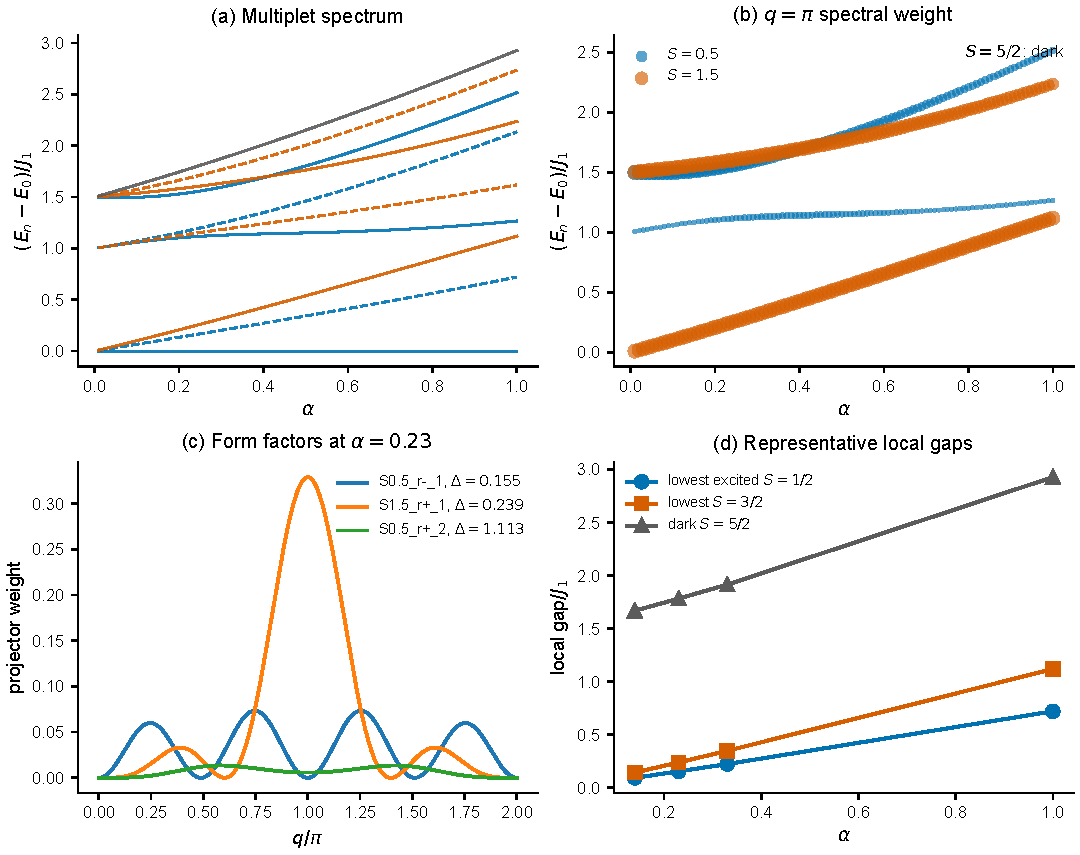
\includegraphics[width=0.98\textwidth]{positive_local_spectral_channels_20260730.pdf}
  \caption{
    通过局域谱权验收的正 $\alpha$ 五聚体激发通道。
    (a) 多重态间隙，实线和虚线分别表示镜像偶、奇宇称；
    (b) 点大小编码 $q=\pi$ 谱权；
    (c) $\alpha=0.23$ 的代表分支形状因子；
    (d) 三个正区代表点和均匀链的局域间隙。
    局域选择定则是有限 $\beta$ 动力学谱的分支先验，不等价于长链色散。
  }
  \label{fig:local-spectral-channels}
\end{figure}

\subsection{受控弱耦合区内局域四重态与两自旋子连续谱分离}

一阶有效 Heisenberg 链的热力学两自旋子连续谱具有
des Cloizeaux--Pearson 下边界
$\omega_{\mathrm L}(q)=\pi J_{\mathrm{eff}}|\sin q|/2$\cite{descloizeaux1962}，
标准两自旋子上边界为
$\omega_{\mathrm U}(q)=\pi J_{\mathrm{eff}}|\sin(q/2)|$。在 $q=\pi$
令上边界 $\pi J_{\mathrm{eff}}$ 与孤立五聚体最低四重态隙相等，可得到形式上的
嵌入阈值。对 $\alpha=0.14,0.23,0.33$，该阈值分别为
$\beta=0.10395,0.17641,0.26469$，对应
$g=\beta/\Delta_{1/2}=1.106,1.138,1.184$。

这些形式阈值均超出当前经多尺寸能隙比标定的经验受控区 $g\leq0.65$。在受控区
边缘，两自旋子上边界只达到局域四重态隙的 $54.9\%$--$58.8\%$。因此，弱耦合
有效理论预言的是低能连续谱与局域四重态之间的有限能量分离，而不是受控的嵌入或
杂化。$\beta=0.5$ 的三个动力学代表点具有 $g=2.24$--$5.32$，不能直接使用
一阶边界给强耦合谱线命名。

\begin{figure}[tb]
  \centering
  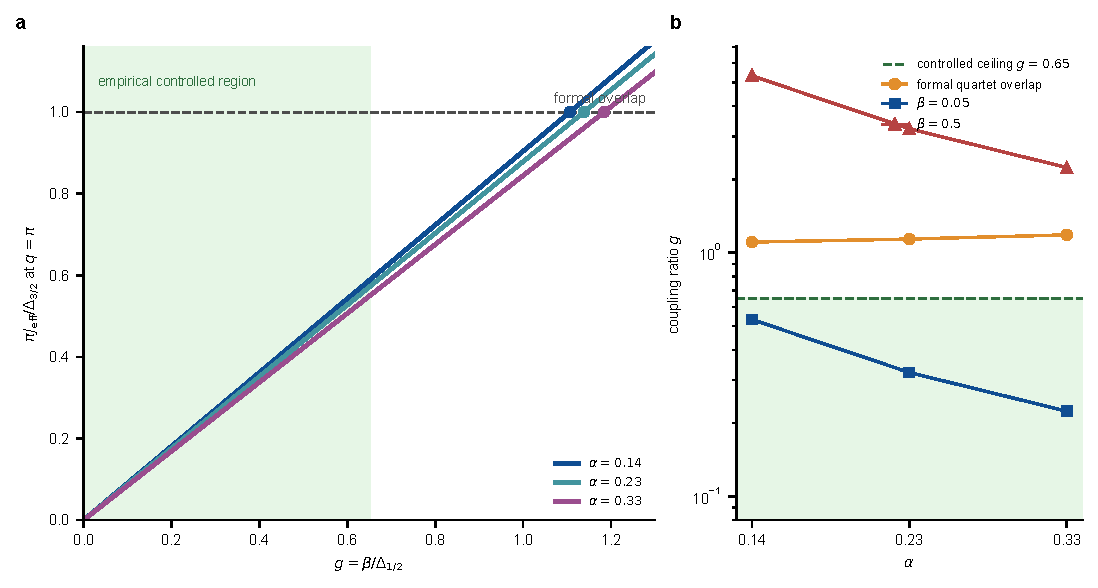
\includegraphics[width=0.98\textwidth]{effective_continuum_overlap_20260730.pdf}
  \caption{
    有效链两自旋子上边界与局域四重态的解析能量比较。
    (a) $q=\pi$ 上边界与四重态隙之比随 $g$ 的变化；绿色区域表示经有限链
    标定的经验受控区。(b) 三个代表点的受控上限、形式重叠阈值及
    $\beta=0.05,0.5$ 所在尺度。形式重叠发生在一阶投影失控后，不能解释为
    已经证明的强耦合杂化。
  }
  \label{fig:continuum-overlap}
\end{figure}

\subsection{修正向量方法通过小系统与长度标定}

在 $L=10$、总 $S^z=0$ 扇区，61 个频率点的修正向量谱与完整精确谱的相对
$L_2$ 误差为 $8.52\times10^{-12}$，积分权重相对误差为
$7.80\times10^{-13}$，最大线性方程相对残差为 $5.82\times10^{-7}$。
该结果验证了 Hamiltonian、动量源、展宽和谱归一化的一致性。

$L=20$ 单点的三档截断序列将残差从 $3.80\times10^{-4}$ 降至
$5.62\times10^{-6}$，最紧两档的谱强度相对差为 $2.33\times10^{-8}$。
$L=40$ 的相同物理点得到残差 $7.48\times10^{-6}$、实际解维数 256、
$1.50$ GiB 峰值内存和 2537 秒修正向量时间。内存不是当前瓶颈，但从
$L=20$ 到 40 的时间倍率为 16.81；在验证相邻频率 warm start 与 checkpoint
恢复前，不能据此直接提交 $L=80$ 频率网格。

\begin{figure}[tb]
  \centering
  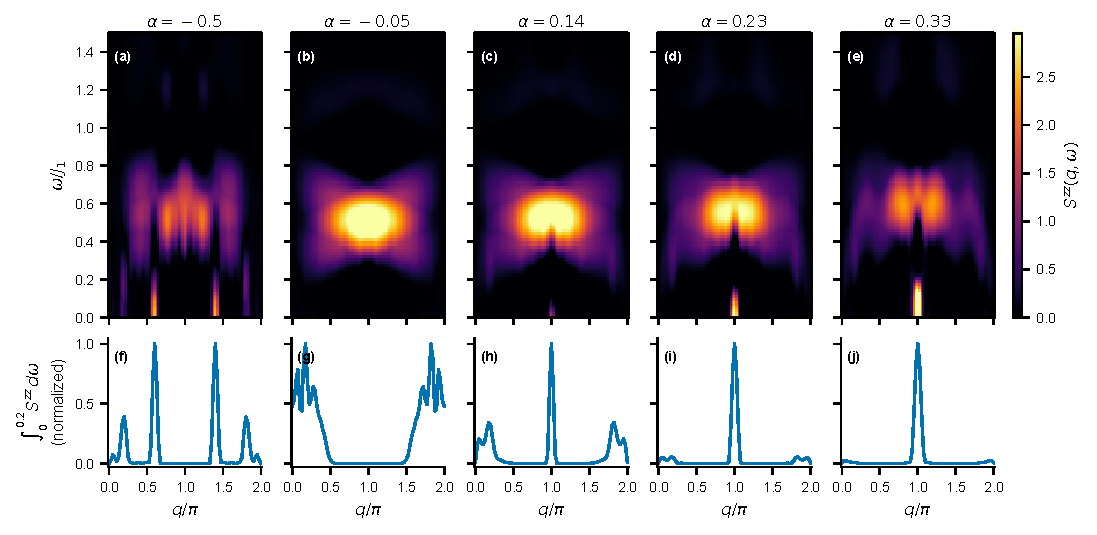
\includegraphics[width=0.88\textwidth]{Sqw_beta_half_pilot_L40_t15.pdf}
  \caption{
    $\beta=0.5$、正 $\alpha$ 代表点的试验性实时动力学结构因子。
    该图只用于定位候选低能权重；正式结论需要生产级修正向量谱、时间步长与
    最大演化时间收敛，以及两种方法的独立交叉检查。
  }
  \label{fig:pilot_dsf}
\end{figure}

\section{讨论}

现有结果最直接的结论是：$\beta=0.5$ 截面不能简单分为负侧普通有隙
Haldane-like 区域和正侧无隙区域。较低能量的负侧延拓态同样具有代数体关联，
但它还保留慢代数弦关联、局域边缘响应和特殊纠缠低能簇。这种组合提示临界体态
与非平庸边缘结构可能共存。

当前证据仍不足以确定负侧的最终普适类。首先，OBC 下
$E(S^z=1)-E(S^z=0)$ 容易受到边缘自由度劈裂污染，不能单独解释为体能隙。
其次，现有弦关联尺寸只到 $L=80$，虽然幂律明显优于指数模型，但还不能排除
更长尺度上的交叉行为。最后，边缘磁化和 Schmidt 低能簇是拓扑解释的重要
支持，却不能替代虚空间投影对称表示。

负侧约 $\alpha=-0.3$ 的波矢变化也需要谨慎处理。它可能对应五站点单胞下的
动量折叠和 Lifshitz 型重分配，但目前没有伴随已测普适量、对称性或拓扑不变量
的突变。类似地，正侧 $\alpha\approx0.17$ 和 $0.30$ 的响应峰反映不同
观测量对有限尺寸交叉尺度的敏感性，而不是自动构成额外相。

后续工作的优先级是：第一，使用更大的 $L$ 和 $t_{\max}$ 验证负侧低能
动力学模式；第二，将普通关联和弦关联扩展到 $L=120,160$；第三，计算 MPS
虚空间投影对称表示；第四，增加其他 $\beta$ 截面后再讨论完整二维相图。

\todo{服务器结果完成后补充 DSF 尺寸和时间标度。}
\todo{补充与无隙 SPT、拓扑 Luttinger liquid 等工作的文献比较。}

\section{结论}

我们研究了自旋 $\frac{1}{2}$ 五聚体 Heisenberg 链在
$\beta=0.5$ 截面上的基态与低能激发。孤立五聚体在
$\alpha=0$ 形成八重低能简并，并在两侧重组为不同的最低自旋多重态。
链模型的多尺寸结果表明，负 $\alpha$ 与正 $\alpha$ 两侧均具有代数普通
自旋关联，但负侧还表现出明显更慢的代数弦关联、局域边缘磁化和特殊纠缠结构。
正侧两个响应峰以及负侧的波矢重分配目前都没有形成独立相界的闭合证据链。

因此，当前最稳妥的相结构描述是：$\alpha=0$ 特殊解耦点分隔一个具有弦与
边缘特征的负侧临界区域和一个常规无隙反铁磁正侧区域。负侧是否属于严格定义的
gapless SPT，以及这一结构如何延伸到完整 $(\alpha,\beta)$ 参数空间，
仍有待更大尺度动力学与虚空间对称性分析。


\printbibliography[title={参考文献}]

\end{document}
